\documentclass{param}

\begin{document}

\numberwithin{table}{section}

%======================================================
% INFORMATIONS DU RAPPORT
%======================================================
\fairepagedegarde

%======================================================
% NUMÉROTATION DES SECTIONS
%======================================================
\renewcommand{\thesection}{\Roman{section}}
\renewcommand{\thesubsection}{\hspace*{0.1cm} \arabic{subsection}}
\renewcommand{\thesubsubsection}{\hspace*{0.2cm} \arabic{subsection}.\arabic{subsubsection}}

%======================================================
% TABLE DES MATIÈRES
%======================================================
\clearpage
\setcounter{page}{2} % commence la numérotation à 2 (page de garde = page 1)
\fairemargesintro % active le style Page X/Y
\tableofcontents

% %======================================================
% % LISTE DES FIGURES
% %======================================================
% \newpage
% \pagestyle{fancy}  % idem pour la liste des figures
% \listoffigures
% \newpage
% \pagestyle{fancy}  % idem pour la liste des figures
% \listoftables

%======================================================
% CORPS DU RAPPORT
%======================================================
\fairemarges

\newpage
\section{Rapport des tests du récepteur JSON}

\subsection{But}
Vérifier la validité d'un fichier JSON et l'intégrité des données reçues.

\subsection{Résumé des tests}
\begin{itemize}
  \item \hyperref[sec:json_example]{Étape 1 : créer un fichier JSON exemple}
  \item \hyperref[sec:json_receiver_code]{Étape 2 : créer un script de test qui importe le récepteur JSON et valide le JSON}
  \item \hyperref[sec:json_sender_code]{Étape 3 : créer un pseudo émetteur qui envoie le JSON au récepteur}
  \item \hyperref[sec:json_compare]{Étape 4 : comparer les données reçues avec les données envoyées}
\end{itemize}

\subsection{Tests}

\subsubsection{fichier json}
\label{sec:json_example}

Dans un premier temps, un fichier JSON exemple a été créé avec les données (spécifié lors de réunions) suivantes :
\begin{itemize}
    \item IMG : buffer de l'image en sortie de la caméra
    \item TEMPÉRATURE : température en degrés Celsius
    \item HUMIDITÉ : humidité en pourcentage
    \item LONGITUDE : longitude
    \item LATITUDE : latitude
    \item HORODATAGE : date et heure
    \item NIVEAU DE BATTERIE : niveau de batterie en pourcentage
\end{itemize}
or, d'autres champs ont été rajoutés pour les besoins de reconstruction d'image
les champs suivant ont été ajoutés :
\begin{itemize}
    \item TYPE : type de format de l'image (jpeg, png, etc.)
    \item WIDTH : largeur de l'image
    \item HEIGHT : hauteur de l'image
\end{itemize}

ce fichier json est disponible à : \texttt{include/code\_json\_receiver/data.json}

\subsubsection{Recepteur JSON}
\label{sec:json_receiver_code}

le récepteur JSON est disponible à : \texttt{include/code\_json\_receiver/receiver.py}

ce script permet de recevoir un objet JSON depuis une page web avec la méthode POST

\subsubsection{Émetteur de test}
\label{sec:json_sender_code}

le récepteur JSON est disponible à : \texttt{include/code\_json\_receiver/emitter.py}

ce script permet d'envoyer l'objet JSON (défini dans \hyperref[sec:json_example]{Étape 1}) à une page web avec la méthode POST

\subsubsection{Comparaison des données}
\label{sec:json_compare}

pour vérifier l'intégrité des données reçues, des JSON simples ont été créés.

JSON envoyé :
\begin{verbatim}
{
  "TEMP": 25,
  "HUMIDITY": 60
}
\end{verbatim}

JSON reçu :
\begin{verbatim}
{
  "TEMP": 25,
  "HUMIDITY": 60
}
\end{verbatim}

\subsection{Validation}

les données reçues sont identiques aux données envoyées, le test est donc concluant.

\subsection{Remarques}
\begin{itemize}
  \item Le récepteur JSON a correctement validé les fichiers JSON envoyés.
\end{itemize}





\newpage
\section{Reconstruction des images}

\subsection{But}
L'objectif de cette étape est de reconstruire les images à partir des données brutes reçues du capteur photo. 

\subsection{Résumé des tests}
\begin{itemize}
  \item \hyperref[sec:formats_images]{étape 1 : lister  les formats d'images produits par le capteur photo}
  \item \hyperref[sec:transformation_images]{étape 2 : mettre en oeuvre la fonction transformant les données brutes en image}
  \item \hyperref[sec:validation_images]{étape 3 : comparer les images reconstruites avec des images de référence}
\end{itemize}

\subsection{Tests}

\subsubsection{Liste des formats d'images}
\label{sec:formats_images}

Le capteur photo utilisé dans le projet peut produire des images dans les formats suivants :
\begin{itemize}
    \item PIXFORMAT\_RGB565 : 2BPP/RGB565 
    \item PIXFORMAT\_YUV422 : 2BPP/YUV422
    \item PIXFORMAT\_YUV420 : 1.5BPP/YUV420
    \item PIXFORMAT\_GRAYSCALE : 1BPP/GRAYSCALE
    \item PIXFORMAT\_JPEG : JPEG/COMPRESSED
    \item PIXFORMAT\_RGB888 : 3BPP/RGB888
    \item PIXFORMAT\_RAW : RAW (tres gros fichier)
    \item PIXFORMAT\_RGB444 : 3BP2P/RGB444
    \item PIXFORMAT\_RGB555 : 3BP2P/RGB555
\end{itemize}

pour les besoins de ce projet, seuls les formats JPEG, RGB565, GRAYSCALE et RGB888 seront retenus.

\subsubsection{Fonction de transformation}
\label{sec:transformation_images}

La fonction de transformation sert à transformer les octets de données brutes en une image exploitable. 
la fonction de transformation est dépendant du format des pixels.

\subsubsection{Comparaison et validation}
\label{sec:validation_images}

Validation pour le format JPEG : 

\begin{figure}[H]
    \centering
    
\includegraphics[width=0.3\textwidth]{include/reconstructeur_image/CIBLE.PNG}
    \caption{Image de référence}
\end{figure}

\begin{figure}[H]
    \centering
    
\includegraphics[width=0.3\textwidth]{include/reconstructeur_image/OUTPUT.PNG}
    \caption{Image reconstruite}
\end{figure}

l'images reconstruite est conforme à l'image de référence. Cependant, il y a une légère différence de luminosité entre les deux images.

\subsection{Remarques}
\begin{itemize}
  \item valider le fonctionnement pour les formats d'image RGB565, GRAYSCALE et RGB888
  \item il faudrait rajouter des corrections de luminosité et de contraste pour améliorer la qualité des images reconstruites
\end{itemize}





\newpage
\section{Base de données SQL}

\subsection{But}
la base de données SQL est le coeur du work package du stockage distant.
Elle doit permettre de stocker les images et leurs métadonnées associées. 

\subsection{Résumé des tests}
\begin{itemize}
  \item étape 1 : création des tables 
  \item étape 2 : création d'entrées dans les tables
  \item étape 3 : insertion d'images (exemple)
  \item étape 4 : affichage des données sur une page web simple
\end{itemize}

\subsection{Tests}

\subsubsection{Tables}
\label{sec:sql_tables}

le stockage distant présente 2 tables :
\begin{itemize}
  \item table "MAIN" : stocke les images reçues et leurs métadonnées
  \item table "STATS" : statistiques d'apparition d'un certain type d'animal (pas encore implémenté)
\end{itemize}

\subsubsection{Point d'entrée}
\label{sec:sql_entree}



\subsubsection{Insertion de données (exemple)}
\label{sec:sql_insertion}

\subsubsection{Affichage web simple}
\label{sec:sql_affichage}

\begin{figure}[H]
    \centering
    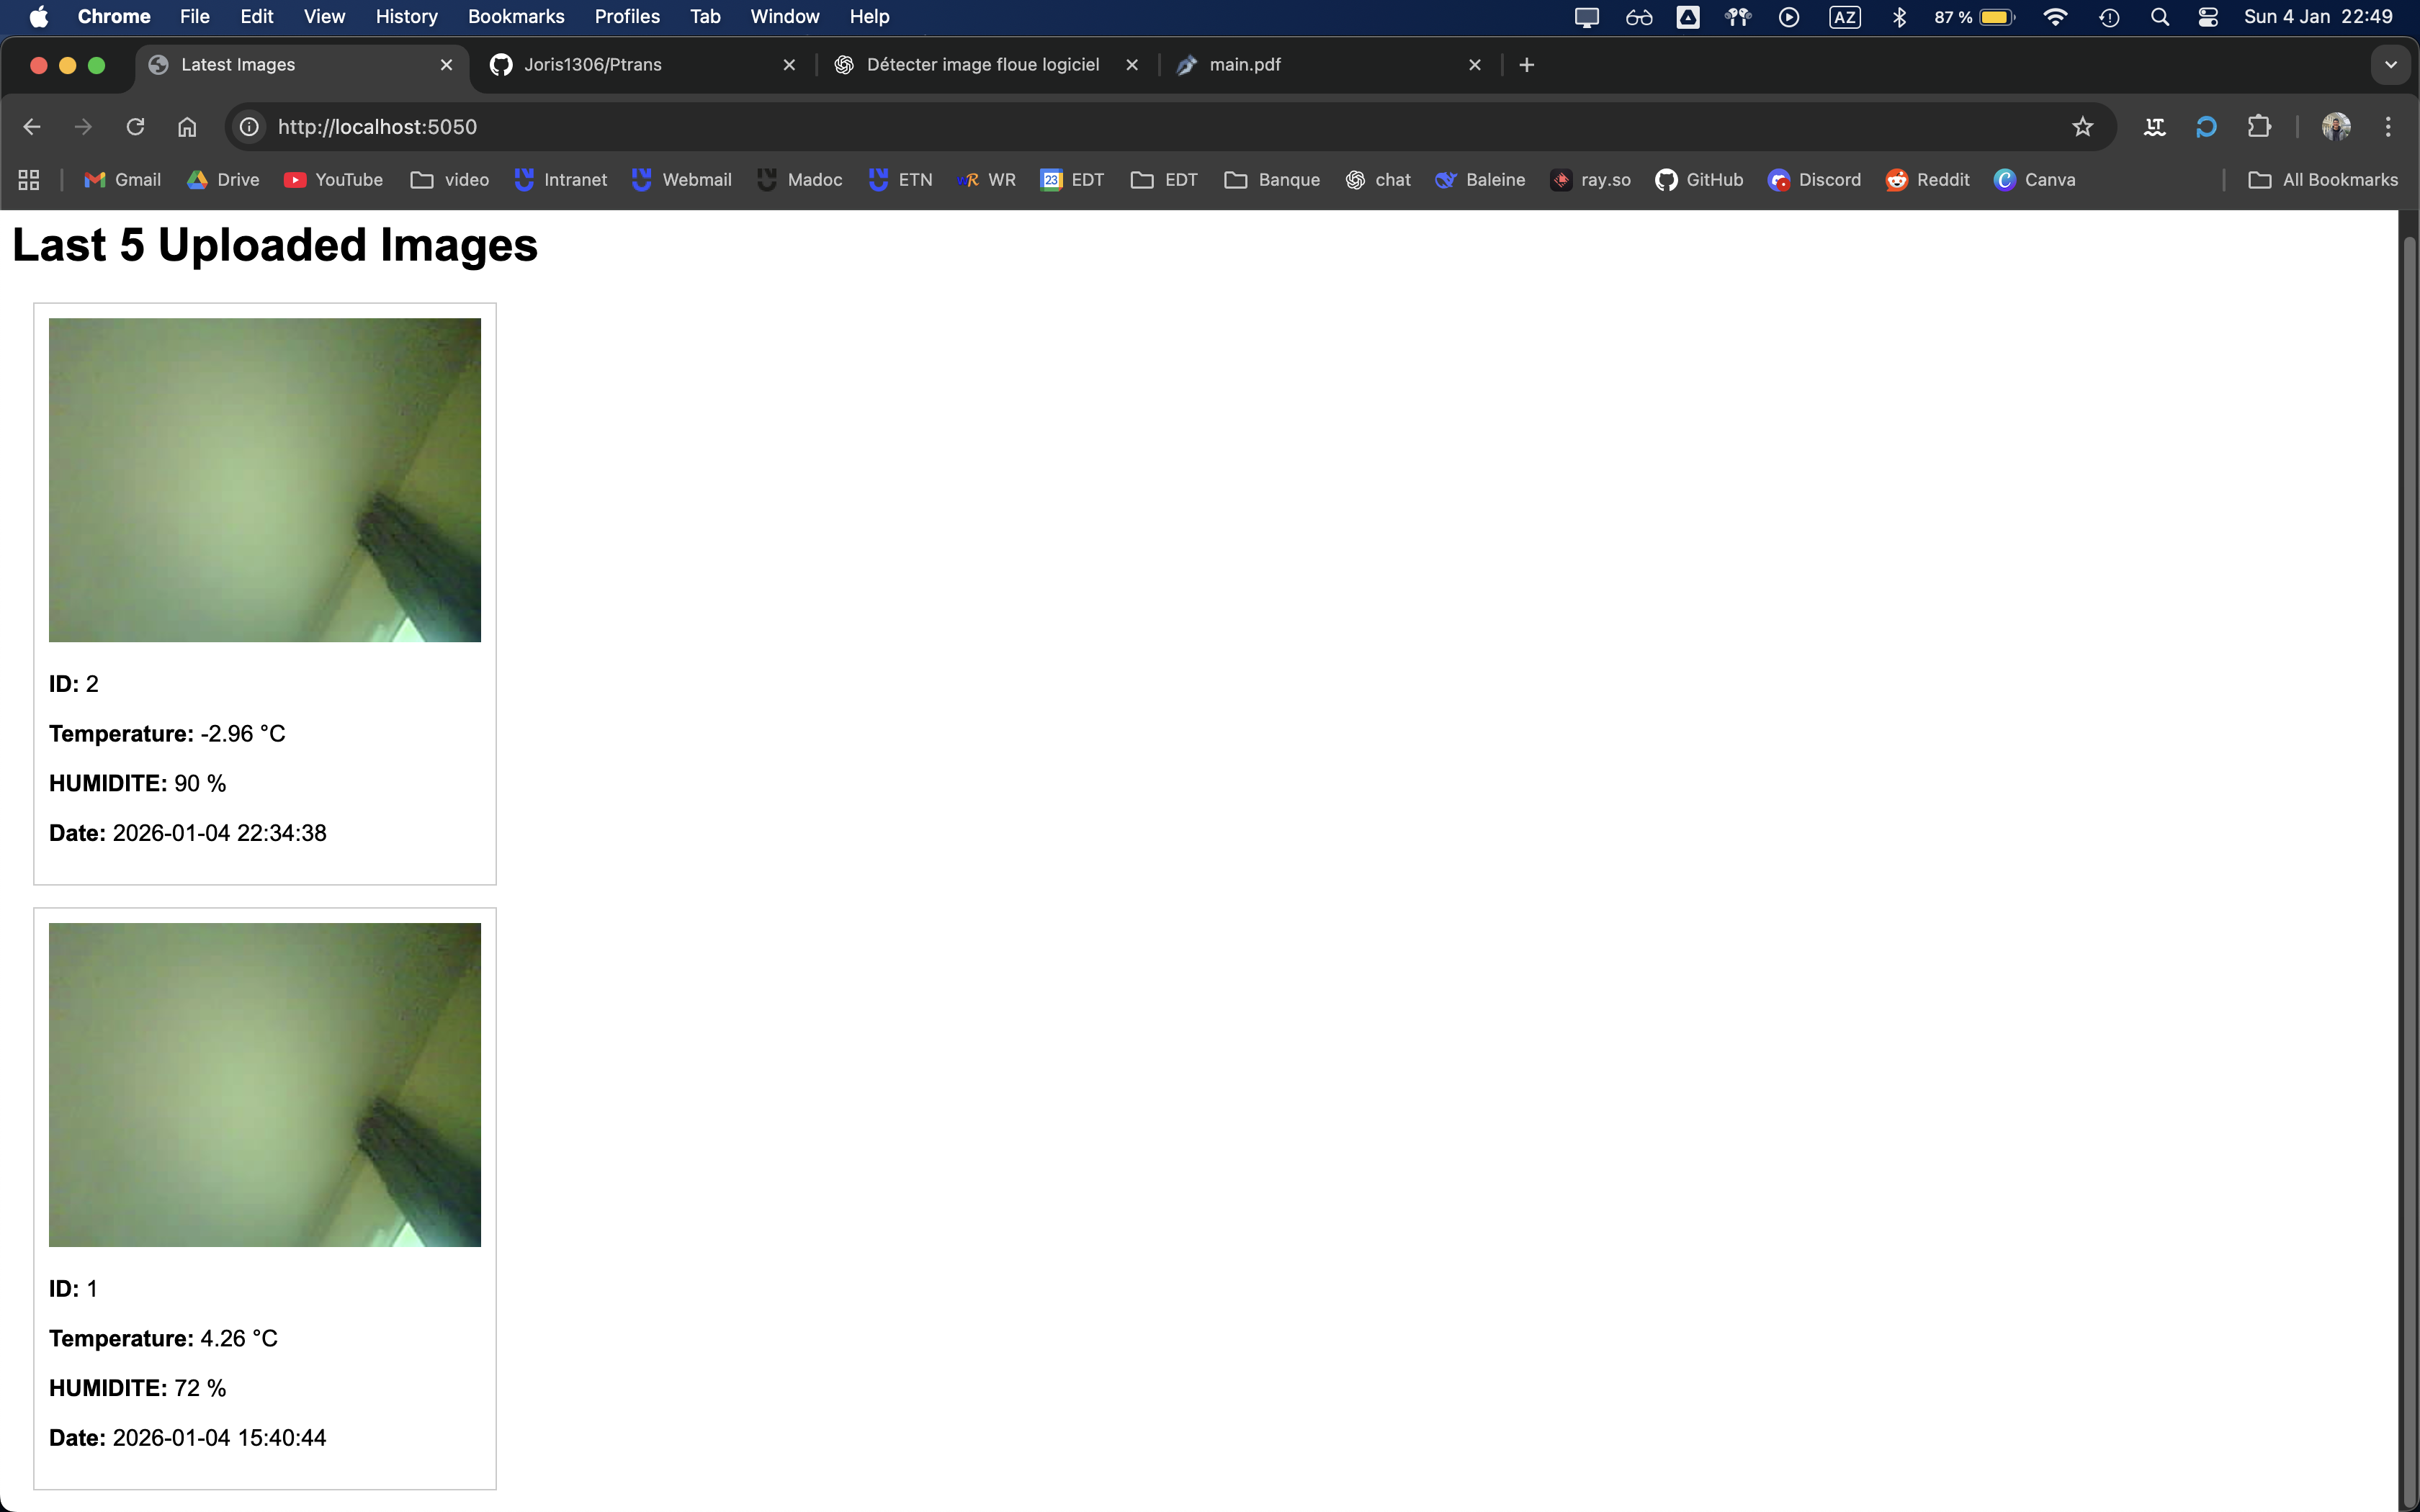
\includegraphics[width=0.8\textwidth]{include/sql_image/webpage.png}
    \caption{Affichage web simple des images stockées dans la base de données SQL}
    \label{fig:sql_web_view}
\end{figure}

\subsection{Remarques}
\begin{itemize}
  \item le WP IHM est lié direcetement au chapitre \ref{sec:sql_affichage}
  \item créer un nouveau point de sortie pour le WP AI CLASSIFICATION
\end{itemize}

% \newpage
% \section{HTTP Viewer (optionnel)}

\subsection{But}

\subsection{Résumé des tests}
\begin{itemize}
  \item étape 1 :
\end{itemize}


\subsection{Remarques}
\begin{itemize}
  \item 
\end{itemize}


%======================================================
% DERNIÈRE PAGE
%======================================================
\label{LastPage} % important pour que Page X/Y fonctionne


%======================================================
% BIBLIOGRAPHIE (optionnelle)
%======================================================
% \newpage
% \bibliographystyle{unsrt}
% \bibliography{bibs/export}

\end{document}